\clearpage

\chapter{\documentName}
\section{\documentName}

\testimonial

The original assignment can be found \pdflink{\AssDir Assignment 2A - Instruction.pdf}{here}, \pdflink{\AssDir Assignment 2A - Code.pdf}{here}, and \pdflink{\AssDir Assignment 2B - Constraint Satisfaction Problem.pdf}{here}.

% Problem 1
\begin{problem}{Problem 1 - CSP Futoshiki}
    \begin{statement}{Problem Statement}
        Futoshiki is a Japanese logic puzzle that is very simple, but can be quite challenging. You are given an $n \times n$ grid, and must place the numbers $1, \dots n$ in the grid such that every 
        row and column has exactly one of each. Additionally, the assignment must satisfy the inequalities placed between some adjacent squares.

        Below is an instance of this problem, for size $n = 4$. Some of the squares have known values, such that the puzzle has a unique solution. (The letters mean nothing to the puzzle, and will be 
        used only as labels with which to refer to certain squares). Note also that inequalities apply only to the two adjacent squares, and do not directly constrain other squares in the row or column.

        \begin{center}
            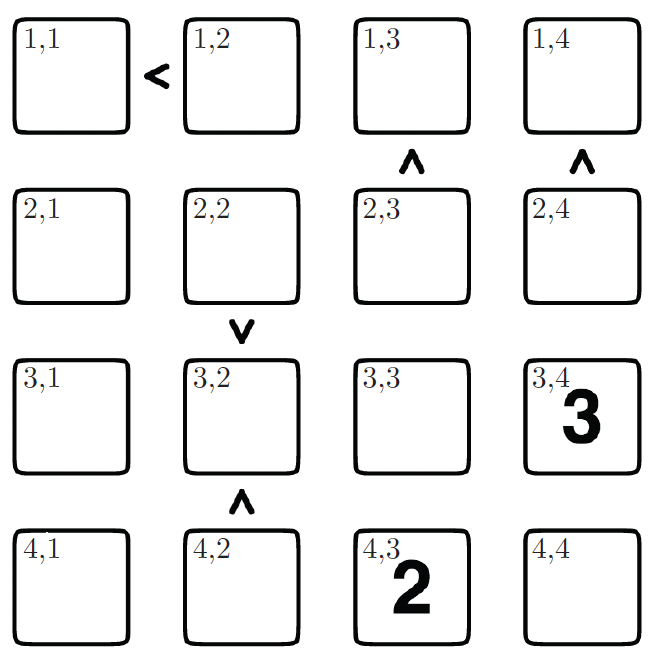
\includegraphics[width=0.3\textwidth]{./Images/Futoshiki Square.png}
        \end{center}

        Let's formulate this puzzle as a CSP. We will use $4^{2}$ variables, one for each cell, with $X_{ij}$ as the variable for the cell in the $i$th row and $j$th column (each cell contains its 
        $i$, $j$ label in the top left corner). The only unary constraints will be those assigning the known initial values to their respective squares (e.g. $X_{34} = 3$).

        \begin{enumerate}[label=\textbf{(\alph*)}]
            \item Complete the formulation of the CSP using only binary constraints (in addition to the unary constraints specificed above). In particular, describe the domains of the variables, and 
            all binary constraints you think are necessary. You do not need to enumerate them all, just describe them using concise mathematical notation. You are not permitted to use $n$-ary constraints 
            where $n \geq 3$.
            \item After enforcing unary constraints, consider the binary constraints involving $X_{14}$ and $X_{24}$. Enforce arc consistency on just these constraints and state the resulting domains 
            for the two variables.
            \item Suppose we enforced unary constraints and ran arc consistency on this CSP, pruning the domains of all variables as much as possible. After this, what is the maximum possible domain 
            size for any variable? [\textit{Hint}: consider the least constrained variable(s); you should \textit{not} have to run every step of arc consistency.]
            \item Suppose we enforced unary constraints and ran arc consistency on the initial CSP in the figure above. What is the maximum possible domain size for a variable adjacent to an inequality?
            \item By inspection of column 2, we find it is necessary that $X_{32} = 1$, despite not having found an assignment to any of the other cells in that column. Would running arc consistency 
            find this requirement? Explain why or why not.
        \end{enumerate}
    \end{statement}

    \clearpage

    \begin{highlight}[Solution - Part A]
        To start, the domain of these cells follows the form of 

        \begin{center}
            \begin{highlightbox}
                D(X_{ij}) = \{1,2,\dots,n\} \text{ for all cells with known values.}
            \end{highlightbox}
        \end{center}
        The unary constraints for this problem are

        \begin{center}
            \begin{highlightbox}
                X_{3,4} = 3 \hspace*{5pt} \text{and} \hspace*{5pt} X_{4,3} = 2.
            \end{highlightbox}
        \end{center}
        The binary constraints for the rows are such that all cells in the row must be unique, for example,

        \begin{center}
            \begin{highlightbox}
                \forall_{i} \forall_{j_{1}} \neq j_{2}, X_{ij_{1}} \neq X_{ij_{2}}.
            \end{highlightbox}
        \end{center}
        The binary constraint for the columns are such that all cells in a column must be unique, for example,

        \begin{center}
            \begin{highlightbox}
                \forall_{j} \forall_{i_{1}} \neq i_{2}, X_{i_{1}j} \neq X_{i_{2}j}.
            \end{highlightbox}
        \end{center}
        The inequality constraint is such that if there exists an inequality between cells, then for example,

        \begin{center}
            \begin{highlightbox}
                X_{i_{1}j_{1}} < X_{i_{2}j_{2}}.
            \end{highlightbox}
        \end{center}
    \end{highlight}

    \begin{highlight}[Solution - Part B]
        If we take for example the first two rows and the final two columns, we first check that $X_{14} \neq X_{24}$. We then prune the domain of $X_{14}$ to remove values that are not possible for 
        $X_{24}$.

        At this point we know that 2,4 and 1,4 cannot be 3. With the constraint in place, this constitutes that 2,4 be greater than 1,4. This means that 2,4 can either be 4 or 2. If 2,4 is 4 then 1,4 can either
        be 2 or 1, but if 2,4 is 2, this means that 1,4 can only be 1.
    \end{highlight}

    \begin{highlight}[Solution - Part C]
        If we take into account the least constrained variables, the maximum domain size should be

        \begin{center}
            \begin{highlightbox}
                n - 1.
            \end{highlightbox}
        \end{center}
    \end{highlight}

    \begin{highlight}[Solution - Part D]
        For a variable that is adjacent to an inequality, the maximum domain size will be reduced, more than likely down to 

        \begin{center}
            \begin{highlightbox}
                n - 2.
            \end{highlightbox}
        \end{center}
    \end{highlight}

    \begin{highlight}[Solution - Part E]
        Arc consistency is not directly going to deduce that $X_{32} = 1$ because arc consistency only prunes inconsistent values and does not specifically deduce assignments. It will specifically
        deduce assignments if other values have been pruned.
    \end{highlight}
\end{problem}

% Problem 2
\begin{problem}{Problem 2 - Course Scheduling}
    \begin{statement}{Problem Statement}
        You are in charge of scheduling for computer science classes that meet Mondays, Wednesdays and Fridays. There are 5 classes that meet on these days and 3 professors who will be teaching these 
        classes. You are constrained by the fact that each professor can only teach one class at a time.

        The classes are:

        \begin{enumerate}
            \item Class 1 - Intro to Programming: meets from 8:00-9:00am
            \item Class 2 - Intro to Artificial Intelligence: meets from 8:30-9:30am
            \item Class 3 - Natural Language Processing: meets from 9:00-10:00am
            \item Class 4 - Computer Vision: meets from 9:00-10:00am
            \item Class 5 - Machine Learning: meets from 10:30-11:30am
        \end{enumerate}

        The professors are:

        \begin{enumerate}
            \item Professor A, who is qualified to teach Classes 1, 2, and 5.
            \item Professor B, who is qualified to teach Classes 3, 4, and 5.
            \item Professor C, who is qualified to teach Classes 1, 3, and 4.
        \end{enumerate}

        \begin{enumerate}[label=\textbf{(\alph*)}]
            \item Formulate this problem as a CSP problem in which there is one variable per class, stating the domains (after enforcing unary constraints), and binary constraints. Constraints should 
            be specified formally and precisely, but may be implicit rather than explicit.
            \item Draw the constraint graph associated with your CSP.
        \end{enumerate}
    \end{statement}
    
    \clearpage

    \begin{highlight}[Solution - Part A]
        The variables in this context are professors A,B, and C and classes $C_{i}$ for each class $i$ from 1 to 5. The classes that can be taught by each professor (the domain) are then

        \begin{itemize}
            \item $D(C_{1}) = \{A,C\}$
            \item $D(C_{2}) = \{A\}$
            \item $D(C_{3}) = \{B,C\}$
            \item $D(C_{4}) = \{B,C\}$
            \item $D(C_{5}) = \{A,B\}$
        \end{itemize}
        The binary constraint for this problem is then

        \begin{center}
            \begin{highlightbox}
                \text{No professor can teach two classes that overlap in time.}
            \end{highlightbox}
        \end{center}
        The unary constraints for this problem are

        \begin{center}
            \begin{highlightenv}[15cm]
                \begin{itemize}
                    \item Class 1 cannot be taught at the same time as class 2 by professor A or C.
                    \item Class 2 cannot be taught at the same time as class 1, 3, or 4 by professor A.
                    \item Class 3 cannot be taught at the same time as class 2 or 4 by professor B or C.
                    \item Class 4 cannot be taught at the same time as class 2 or 3 by professor B or C.
                    \item Class 5 does not have any specific constraints of when it can be taught by professor A or B.
                \end{itemize}
            \end{highlightenv}
        \end{center}
    \end{highlight}

    \begin{highlight}[Solution - Part B]
        The constraint graph for this problem can be found below.

        \begin{center}
            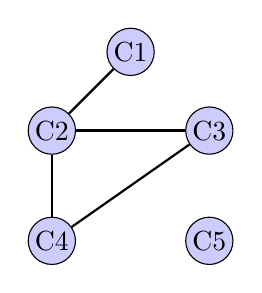
\begin{tikzpicture}
                [node/.style={circle, draw, fill=blue!20, minimum size=6mm, inner sep=0pt}, edge/.style={draw, thick}]
                % Define nodes
                \node[node] (1) at (0,0) {C1};
                \node[node] (2) at (-1,-1) {C2};
                \node[node] (3) at (1,-1) {C3};
                \node[node] (4) at (-1,-2.4) {C4};
                \node[node] (5) at (1,-2.4) {C5};
                % Define edges
                \draw[edge] (1) -- (2);
                \draw[edge] (2) -- (3);
                \draw[edge] (2) -- (4);
                \draw[edge] (3) -- (4);
            \end{tikzpicture}
        \end{center}
        The nodes in the above image represent classes and the edges represent constraints between the classes. This means if an edge exists between the two classes, these two classes cannot be taught
        at the same time as one another.

        In the above image, class 1 cannot be taught at the same time as class 2, class 2 cannot be taught at the same time as class 1, 3, or 4, class 3 cannot be taught at the same time as class 2 or 4,
        and class 4 cannot be taught at the same time as class 2 or 3. Class 5 does not have any conflicts with the other classes.
    \end{highlight}
\end{problem}

% Problem 3
\begin{problem}{Problem 3 - CSP: Air Traffic Control}
    \begin{statement}{Problem Statement}
        We have five planes: A, B, C, D, and E and two runways: international and domestic. We would like to schedule a time slot and runway for each aircraft to \textbf{either} land or take off. We 
        have four time slots: $\{1, 2, 3, 4\}$ for each runway, during which we can schedule a landing or take off of a plane. We must find an assignment that meets the following constraints:

        \begin{itemize}
            \item Plane B has lost an engine and must land in time slot 1.
            \item Plane D can only arrive at the airport to land during or after time slot 3.
            \item Plane A is running low on fuel but can last until at most time slot 2.
            \item Plane D must land before plane C takes off, because some passengers must transfer from D to C.
            \item No two aircrafts can reserve the same time slot for the same runway.
        \end{itemize}

        \begin{enumerate}[label=\textbf{(\alph*)}]
            \item Complete the formulation of this problem as a CSP in terms of variables, domains, and constraints (both unary and binary). Constraints should be expressed implicitly using mathematical 
            or logical notation rather than with words.
            \item For the following subparts, we add the following two constraints:
            \begin{itemize}
                \item Planes A, B, and C cater to international flights and can only use the international runway.
                \item Planes D and E cater to domestic flights and can only use the domestic runway.
            \end{itemize}
            \begin{enumerate}[label=\textbf{(\roman*)}]
                \item With the addition of the two constraints above, we completely reformulate the CSP and draw the constraint graph.
                \item What are the domains of the variables after enforcing arc-consistency? Begin by enforcing unary constraints. (Cross out values that are no longer in the domain.)
                \begin{equation*}
                    \begin{array}{c|cccc}
                        A & 1 & 2 & 3 & 4 \\
                        B & 1 & 2 & 3 & 4 \\
                        C & 1 & 2 & 3 & 4 \\
                        D & 1 & 2 & 3 & 4 \\
                        E & 1 & 2 & 3 & 4 \\
                    \end{array}
                \end{equation*}
                \item Arc-consistency can be rather expensive to enforce, and we believe that we can obtain faster solutions using only forward-checking on our variable assignments. Using the Minimum 
                Remaining Values heuristic, perform backtracking search on the graph, breaking ties by picking lower values and characters first. List the (variable; assignment) pairs in the order 
                they occur (including the assignments that are reverted upon reaching a dead end). Enforce unary constraints before starting the search.
                \begin{equation*}
                    \begin{array}{c|cccc}
                        A & 1 & 2 & 3 & 4 \\
                        B & 1 & 2 & 3 & 4 \\
                        C & 1 & 2 & 3 & 4 \\
                        D & 1 & 2 & 3 & 4 \\
                        E & 1 & 2 & 3 & 4 \\
                    \end{array}
                \end{equation*}
            \end{enumerate}
        \end{enumerate}
    \end{statement}

    \clearpage

    \begin{highlight}[Solution - Part A]
        The variables for each plane $i$ have a runway assignment $X_{i}$. The domains correlate to the time slots $\{1,2,3,4\}$ and the constraints are 

        \begin{center}
            \begin{highlightbox}
                \text{\textbf{Binary}: No two planes can use the runway at the same time.}
            \end{highlightbox}
        \end{center}
        For the Unary constraints, these are when the planes are allowed to land:

        \begin{center}
            \begin{highlightenv}[10cm]
                \begin{itemize}
                    \item $X_{A} \leq 2$
                    \item $X_{B} = 1$
                    \item $X_{D} \geq 3$
                    \item $X_{D} < X_{C}$
                \end{itemize}
                \vspace*{1em}
                Or formally
                \begin{equation*}
                    \forall I,J \in \{A,B,C,D,E\}, I \neq J, X_{I} \neq X_{J}
                \end{equation*}
            \end{highlightenv}
        \end{center}
    \end{highlight}

    \begin{highlight}[Solution - Part B]
        \subsubsection*{Part (i)}

        The domain and binary constraints do not change in this context. The only thing that changes from part (A) are the unary constraints. The unary constraints are then \vspace*{1em}

        \begin{center}
            \begin{highlightenv}[10cm]
                \begin{itemize}
                    \item $X_{A} \leq 2$
                    \item $X_{B} = 1$
                    \item $X_{D} \geq 3$
                    \item $X_{D} < X_{C}$
                    \item Planes A,B, and C must use international runway.
                    \item Planes D and E must use domestic runway.
                \end{itemize}
            \end{highlightenv}
        \end{center}

        The constraint graph would then look like the following.

        \begin{center}
            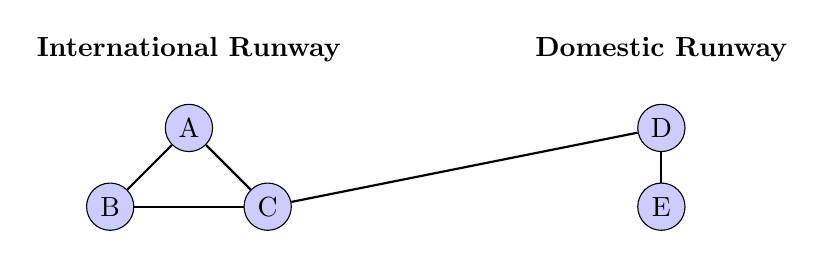
\begin{tikzpicture}
                [node/.style={circle, draw, fill=blue!20, minimum size=6mm, inner sep=0pt}, edge/.style={draw, thick}]
                % Define nodes
                \node[draw=none,fill=none] (Title 1) at (-3,1) {\textbf{International Runway}};
                \node[node] (A) at (-3,0) {A};
                \node[node] (B) at (-4,-1) {B};
                \node[node] (C) at (-2,-1) {C};
                \node[draw=none,fill=none] (Title 2) at (3,1) {\textbf{Domestic Runway}};
                \node[node] (D) at (3,0) {D};
                \node[node] (E) at (3,-1) {E};
                % Define edges
                \draw[edge] (A) -- (B);
                \draw[edge] (A) -- (C);
                \draw[edge] (B) -- (C);
                \draw[edge] (D) -- (C);
                \draw[edge] (D) -- (E);
            \end{tikzpicture}
        \end{center}
        Nodes in this graph represent planes and edges represent constraints between the planes.

        \subsubsection*{Part (ii)}

        After enforcing arc consistency with the aforementioned constraints, the domains of each plane are then:

        \begin{center}
            \begin{highlightenv}[7.5cm]
                \begin{equation*}
                    \begin{array}{c|cccc}
                        A & \cancel{1} & 2 & \cancel{3} & \cancel{4} \\
                        B & 1 & \cancel{2} & \cancel{3} & \cancel{4} \\
                        C & \cancel{1} & \cancel{2} & \cancel{3} & 4 \\
                        D & \cancel{1} & \cancel{2} & 3 & \cancel{4} \\
                        E & 1 & 2 & \cancel{3} & 4 \\
                    \end{array}
                \end{equation*}
            \end{highlightenv}
        \end{center}

        \subsubsection*{Part (iii)}

        To address this we first start with the most constrained variable, plane B:

        \begin{itemize}
            \item $X_{B} = 1$ (Plane B must land first)
            \item We then perform forward checking and remove this time from all the planes landing on the international runway
            \begin{itemize}
                \item $D(X_{A}) = \{2\}$
                \item $D(X_{C}) = \{2,3,4\}$
            \end{itemize}
            \item Next, we enforce the time in which plane A must land
            \begin{itemize}
                \item $X_{A} = 2$
            \end{itemize}
            \item We then remove this time from the same international runway planes
            \begin{itemize}
                \item $D(X_{C}) = \{3,4\}$
            \end{itemize}
            \item The next most constrained variable is plane D since it must land before plane C takes off. Since the only possible values at this point for plane C are 3 and 4 this means that plane D
            must land at time 3
            \begin{itemize}
                \item $X_{D} = 3$
            \end{itemize}
            \item We then remove this time slot from plane C and we have
            \begin{itemize}
                \item $X_{C} = 4$
            \end{itemize}
            \item The next most constrained variable is then plane E and it must land at a different time than plane D leaving the domain for plane E as
            \begin{itemize}
                \item $D(X_{E}) = \{1,2,4\}$
            \end{itemize}
        \end{itemize}
        The order in which the planes are assigned times is then

        \begin{center}
            \begin{highlightbox}
                (B,1) \rightarrow (A,2) \rightarrow (D,3) \rightarrow (C,4) \rightarrow (E, \{1,2,4\}).
            \end{highlightbox}
        \end{center}
    \end{highlight}

\end{problem}

% Problem 4 - 2A Question 1
\begin{problem}{Problem 4 - 2A Question 1}
    \begin{statement}{Problem Statement}
        Modify your code for uniform-cost search from Homework 1 so that it provides optionally as output the number of nodes expanded in completing the search.

        Include a new optional logical (True/False) argument \texttt{return\_nexp}, so your function calls to the new uniform cost search will look like: \texttt{uniform\_cost(start, goal, state\_graph, return\_cost, return\_nexp)}.

        \begin{itemize}
            \item If \texttt{return\_nexp} is True, then the last output in the output tuple should be the number of nodes expanded.
            \item If \texttt{return\_nexp} is False, then the code should behave exactly as it did in Homework 1.
        \end{itemize}

        Then, verify that your revised codes are working by checking Neal's optimal route from New York to Chicago. Include the number of nodes expanded and the path cost (using \texttt{map\_distances}).
    \end{statement}

    \begin{highlight}[Solution]
    \begin{code}[Python]
    import numpy as np
    import heapq
    import unittest
    
    def path(previous, s): 
        '''
        `previous` is a dictionary chaining together the predecessor state that led to each state
        `s` will be None for the initial state
        otherwise, start from the last state `s` and recursively trace `previous` back to the initial state,
        constructing a list of states visited as we go
        '''
        if s is None:
            return []
        else:
            return path(previous, previous[s])+[s]
    
    def pathcost(path, step_costs):
        '''
        add up the step costs along a path, which is assumed to be a list output from the `path` function above
        '''
        cost = 0
        for s in range(len(path)-1):
            cost += step_costs[path[s]][path[s+1]]
        return cost
    
    map_distances = dict(
        chi=dict(det=283, cle=345, ind=182),
        cle=dict(chi=345, det=169, col=144, pit=134, buf=189),
        ind=dict(chi=182, col=176),
        col=dict(ind=176, cle=144, pit=185),
        det=dict(chi=283, cle=169, buf=256),
        buf=dict(det=256, cle=189, pit=215, syr=150),
        pit=dict(col=185, cle=134, buf=215, phi=305, bal=247),
        syr=dict(buf=150, phi=253, new=254, bos=312),
        bal=dict(phi=101, pit=247),
        phi=dict(pit=305, bal=101, syr=253, new=97),
        new=dict(syr=254, phi=97, bos=215, pro=181),
        pro=dict(bos=50, new=181),
        bos=dict(pro=50, new=215, syr=312, por=107),
        por=dict(bos=107))
    
    sld_providence = dict(
        chi=833,
        cle=531,
        ind=782,
        col=618,
        det=596,
        buf=385,
        pit=458,
        syr=253,
        bal=325,
        phi=236,
        new=157,
        pro=0,
        bos=38,
        por=136)
    
    # Solution:
    
    """ Frontier_PQ - Implements a priority queue ordered by path cost for uniform cost search
        Methods:
            __init__ - Initializes an empty priority queue
            is_empty - Checks if the priority queue is empty
            put - Adds an item with a specified priority to the priority queue
            get - Removes and returns the item with the lowest priority from the priority queue
        Algorithm:
            * __init__ initializes an empty list to represent the priority queue
            * is_empty returns True if the list is empty, otherwise False
            * put uses heapq.heappush to add an item to the priority queue with the given priority
            * get uses heapq.heappop to remove and return the item with the lowest priority
        Output:
            * is_empty returns a boolean indicating whether the priority queue is empty
            * put does not return a value
            * get returns the item with the lowest priority
    """
    class Frontier_PQ:
        ''' frontier class for uniform search, ordered by path cost '''
        # add your code here
        def __init__(self):
            self.elements = []
        def is_empty(self):
            return len(self.elements) == 0
        def put(self, item, priority):
            heapq.heappush(self.elements, (priority, item))
        def get(self):
            return heapq.heappop(self.elements)
    
    """ uniform_cost - Performs a Uniform Cost Search (UCS) on the state graph for the path between a start and goal.
        Input:
            start - Node that represents the start of the path.
            goal - Node that represents the desired end point of the path.
            state_graph - Dictionary representing the graph being searched, with costs for each edge.
            return_cost - Boolean value that indicates whether to return the cost of the path.
            return_nexp - Boolean value that indicates whether to return the number of nodes expanded.
        Algorithm:
            * Initialize a Frontier_PQ instance and add the start node with a priority of 0.
            * Initialize a dictionary of previous nodes with the start node set to None.
            * Initialize a dictionary to keep track of the cost to reach each node with the start node set to 0.
            * Initialize a counter to keep track of the number of nodes expanded (nodes_expanded) and set it to 0.
            * While the priority queue is not empty:
                * Get the node with the lowest cost from the priority queue.
                * If the current node is the goal:
                    * Update the path to the goal using the previous nodes and the goal.
                    * Calculate the cost if return_cost is True.
                    * If return_cost is True:
                        * If return_nexp is True, return the path to the goal, the cost, and the number of nodes expanded.
                        * Otherwise, return the path to the goal and the cost.
                    * If return_cost is False:
                        * If return_nexp is True, return the path to the goal and the number of nodes expanded.
                        * Otherwise, just return the path to the goal.
                * Increment the nodes_expanded counter.
                * Iterate over the neighbors of the current node:
                    * Calculate the new cost to reach each neighbor.
                    * If the neighbor has not been visited or the new cost is lower than the recorded cost:
                        * Update the cost to reach the neighbor.
                        * Add the neighbor to the priority queue with the new cost as priority.
                        * Update the previous nodes with the current node.
            * If the goal is not reachable:
                * If return_cost is True:
                    * If return_nexp is True, return (None, 0, nodes_expanded).
                    * Otherwise, return (None, 0).
                * If return_cost is False:
                    * If return_nexp is True, return (None, nodes_expanded).
                    * Otherwise, return None.
        Output:
            Returns the path to the goal.
            If return_cost is True, also returns the cost of the path.
            If return_nexp is True, also returns the number of nodes expanded.
    """
    def uniform_cost(start, goal, state_graph, return_cost=False, return_nexp=True):
        frontier = Frontier_PQ()
        frontier.put(start, 0)
        previous = {start: None}
        cost_so_far = {start: 0}
        nodes_expanded = 0
        while not frontier.is_empty():
            current_priority, current = frontier.get()
            if current == goal:
                path_to_goal = path(previous, goal)
                if return_cost:
                    cost = pathcost(path_to_goal, state_graph)
                    if return_nexp:
                        return path_to_goal, cost, nodes_expanded
                    else:
                        return path_to_goal, cost
                else:
                    if return_nexp:
                        return path_to_goal, nodes_expanded
                    else:
                        return path_to_goal
            nodes_expanded += 1
            for neighbor in state_graph[current]:
                new_cost = cost_so_far[current] + state_graph[current][neighbor]
                if neighbor not in cost_so_far or new_cost < cost_so_far[neighbor]:
                    cost_so_far[neighbor] = new_cost
                    priority = new_cost
                    frontier.put(neighbor, priority)
                    previous[neighbor] = current
        if return_cost:
            if return_nexp:
                return None, 0, nodes_expanded
            else:
                return None, 0
        else:
            if return_nexp:
                return None, nodes_expanded
            else:
                return None
    \end{code}
    \end{highlight}
\end{problem}

% Problem 5 - 2A Question 2
\begin{problem}{Problem 5 - 2A Question 2}
    \begin{statement}{Problem Statement}
        Define a function to take as an argument the state that Neal is in (city on our graphs), and return as output the value of the straight-line distance heuristic, between Neal's state and Providence.

        Note that your function should be quite short, and amounts to looking up the proper value from the \texttt{sld\_providence} dictionary defined in the helper functions. Call this function \texttt{heuristic\_sld\_providence}.
    \end{statement}

    \begin{highlight}[Solution]
    \begin{code}[Python]
    sld_providence = dict(
        chi=833,
        cle=531,
        ind=782,
        col=618,
        det=596,
        buf=385,
        pit=458,
        syr=253,
        bal=325,
        phi=236,
        new=157,
        pro=0,
        bos=38,
        por=136)
    
    """ heuristic_sld_providence - Returns the straight-line distance heuristic between the given state (city) and Providence.
        Input:
            state - The current city/state as a string.
        Output:
            The straight-line distance from the given state to Providence as an integer.
    """
    def heuristic_sld_providence(state):
        return sld_providence[state]
    \end{code}
    \end{highlight}
\end{problem}

% Problem 6 - 2A Question 3
\begin{problem}{Problem 6 - 2A Question 3}
    \begin{statement}{Problem Statement}
        We are finally ready to help Neal use his knowledge of straight-line distances from various cities to Providence to inform his family's route to move from Chicago to Providence!

        Modify your uniform-cost search codes from 1.1 even further so that they now perform A* search, using as the heuristic function the straight-line distance to Providence.

        Provide heuristic as an additional argument, which should just be the function to call within the A* code. So your call to the A routine should look like: \texttt{astar\_search(start, goal, state\_graph, heuristic, return\_cost, return\_nexp)}. 
        (This kind of modular programming will make it much easier to swap in alternative heuristic functions later, and also helps to facilitate debugging if something goes wrong.)
    \end{statement}

    \begin{highlight}[Solution]
    \begin{code}[Python]
    import numpy as np
    import heapq
    import unittest
    
    def path(previous, s): 
        '''
        `previous` is a dictionary chaining together the predecessor state that led to each state
        `s` will be None for the initial state
        otherwise, start from the last state `s` and recursively trace `previous` back to the initial state,
        constructing a list of states visited as we go
        '''
        if s is None:
            return []
        else:
            return path(previous, previous[s])+[s]
    
    def pathcost(path, step_costs):
        '''
        add up the step costs along a path, which is assumed to be a list output from the `path` function above
        '''
        cost = 0
        for s in range(len(path)-1):
            cost += step_costs[path[s]][path[s+1]]
        return cost
    
    map_distances = dict(
        chi=dict(det=283, cle=345, ind=182),
        cle=dict(chi=345, det=169, col=144, pit=134, buf=189),
        ind=dict(chi=182, col=176),
        col=dict(ind=176, cle=144, pit=185),
        det=dict(chi=283, cle=169, buf=256),
        buf=dict(det=256, cle=189, pit=215, syr=150),
        pit=dict(col=185, cle=134, buf=215, phi=305, bal=247),
        syr=dict(buf=150, phi=253, new=254, bos=312),
        bal=dict(phi=101, pit=247),
        phi=dict(pit=305, bal=101, syr=253, new=97),
        new=dict(syr=254, phi=97, bos=215, pro=181),
        pro=dict(bos=50, new=181),
        bos=dict(pro=50, new=215, syr=312, por=107),
        por=dict(bos=107))
    
    sld_providence = dict(
        chi=833,
        cle=531,
        ind=782,
        col=618,
        det=596,
        buf=385,
        pit=458,
        syr=253,
        bal=325,
        phi=236,
        new=157,
        pro=0,
        bos=38,
        por=136)
    
    # Solution:
    
    """ heuristic_sld_providence - Returns the straight-line distance heuristic between the given state (city) and Providence.
        Input:
            state - The current city/state as a string.
        Output:
            The straight-line distance from the given state to Providence as an integer.
    """
    def heuristic_sld_providence(state):
        return sld_providence[state]
    
    """ Frontier_PQ - Implements a priority queue ordered by path cost for uniform cost search
        Methods:
            __init__ - Initializes an empty priority queue
            is_empty - Checks if the priority queue is empty
            put - Adds an item with a specified priority to the priority queue
            get - Removes and returns the item with the lowest priority from the priority queue
        Algorithm:
            * __init__ initializes an empty list to represent the priority queue
            * is_empty returns True if the list is empty, otherwise False
            * put uses heapq.heappush to add an item to the priority queue with the given priority
            * get uses heapq.heappop to remove and return the item with the lowest priority
        Output:
            * is_empty returns a boolean indicating whether the priority queue is empty
            * put does not return a value
            * get returns the item with the lowest priority
    """
    class Frontier_PQ:
        ''' frontier class for uniform search, ordered by path cost '''
        # add your code here
        def __init__(self):
            self.elements = []
        def is_empty(self):
            return len(self.elements) == 0
        def put(self, item, priority):
            heapq.heappush(self.elements, (priority, item))
        def get(self):
            return heapq.heappop(self.elements)
        
    # Solution:
    """ astar_search - Performs an A* Search on the state graph for the path between a start and goal.
        Input:
            start - Node that represents the start of the path.
            goal - Node that represents the desired end point of the path.
            state_graph - Dictionary representing the graph being searched, with costs for each edge.
            heuristic - Function to estimate the cost from a state to the goal.
            return_cost - Boolean value that indicates whether to return the cost of the path.
            return_nexp - Boolean value that indicates whether to return the number of nodes expanded.
        Algorithm:
            * Initialize a Frontier_PQ instance and add the start node with a priority of 0.
            * Initialize a dictionary of previous nodes with the start node set to None.
            * Initialize a dictionary to keep track of the cost to reach each node with the start node set to 0.
            * Initialize a counter to keep track of the number of nodes expanded (nodes_expanded) and set it to 0.
            * While the priority queue is not empty:
                * Get the node with the lowest cost from the priority queue.
                * Increment the nodes_expanded counter.
                * If the current node is the goal:
                    * Update the path to the goal using the previous nodes and the goal.
                    * Calculate the cost if return_cost is True.
                    * If return_cost is True:
                        * If return_nexp is True, return the path to the goal, the cost, and the number of nodes expanded.
                        * Otherwise, return the path to the goal and the cost.
                    * If return_cost is False:
                        * If return_nexp is True, return the path to the goal and the number of nodes expanded.
                        * Otherwise, just return the path to the goal.
                * Iterate over the neighbors of the current node:
                    * Calculate the new cost to reach each neighbor.
                    * If the neighbor has not been visited or the new cost is lower than the recorded cost:
                        * Update the cost to reach the neighbor.
                        * Calculate the priority by adding the heuristic value to the new cost.
                        * Add the neighbor to the priority queue with the new priority.
                        * Update the previous nodes with the current node.
            * If the goal is not reachable:
                * If return_cost is True:
                    * If return_nexp is True, return (None, 0, nodes_expanded).
                    * Otherwise, return (None, 0).
                * If return_cost is False:
                    * If return_nexp is True, return (None, nodes_expanded).
                    * Otherwise, return None.
        Output:
            Returns the path to the goal.
            If return_cost is True, also returns the cost of the path.
            If return_nexp is True, also returns the number of nodes expanded.
    """
    def astar_search(start, goal, state_graph, heuristic, return_cost=False, return_nexp=False):
        frontier = Frontier_PQ()
        frontier.put(start, 0)
        previous = {start: None}
        cost_so_far = {start: 0}
        nodes_expanded = 0
        while not frontier.is_empty():
            current_priority, current = frontier.get()
            nodes_expanded += 1
            if current == goal:
                path_to_goal = path(previous, goal)
                if return_cost:
                    cost = pathcost(path_to_goal, state_graph)
                    if return_nexp:
                        return path_to_goal, cost, nodes_expanded
                    else:
                        return path_to_goal, cost
                else:
                    if return_nexp:
                        return path_to_goal, nodes_expanded
                    else:
                        return path_to_goal
            for neighbor in state_graph[current]:
                new_cost = cost_so_far[current] + state_graph[current][neighbor]
                if neighbor not in cost_so_far or new_cost < cost_so_far[neighbor]:
                    cost_so_far[neighbor] = new_cost
                    priority = new_cost + heuristic(neighbor)
                    frontier.put(neighbor, priority)
                    previous[neighbor] = current
        if return_cost:
            if return_nexp:
                return None, 0, nodes_expanded
            else:
                return None, 0
        else:
            if return_nexp:
                return None, nodes_expanded
            else:
                return None
    \end{code}
    \end{highlight}
\end{problem}

% Problem 7 - 2A Question 4
\begin{problem}{Problem 7 - 2A Question 4}
    \begin{statement}{Problem Statement}
        Print the the following using your code:

        \begin{enumerate}
            \item The optimal path.
            \item The optimal path cost (miles traveled).
            \item The number of states expanded during the A* search.
        \end{enumerate}

        Additionally, print how many states must be expanded to find the optimal path from Buffalo to Providence using the regular old uniform-cost search algorithm from 1.1.
    \end{statement}

    \begin{highlight}[Solution]
    \begin{code}[Python]
    import numpy as np
    import heapq
    import unittest
    
    def path(previous, s): 
        '''
        `previous` is a dictionary chaining together the predecessor state that led to each state
        `s` will be None for the initial state
        otherwise, start from the last state `s` and recursively trace `previous` back to the initial state,
        constructing a list of states visited as we go
        '''
        if s is None:
            return []
        else:
            return path(previous, previous[s])+[s]
    
    def pathcost(path, step_costs):
        '''
        add up the step costs along a path, which is assumed to be a list output from the `path` function above
        '''
        cost = 0
        for s in range(len(path)-1):
            cost += step_costs[path[s]][path[s+1]]
        return cost
    
    map_distances = dict(
        chi=dict(det=283, cle=345, ind=182),
        cle=dict(chi=345, det=169, col=144, pit=134, buf=189),
        ind=dict(chi=182, col=176),
        col=dict(ind=176, cle=144, pit=185),
        det=dict(chi=283, cle=169, buf=256),
        buf=dict(det=256, cle=189, pit=215, syr=150),
        pit=dict(col=185, cle=134, buf=215, phi=305, bal=247),
        syr=dict(buf=150, phi=253, new=254, bos=312),
        bal=dict(phi=101, pit=247),
        phi=dict(pit=305, bal=101, syr=253, new=97),
        new=dict(syr=254, phi=97, bos=215, pro=181),
        pro=dict(bos=50, new=181),
        bos=dict(pro=50, new=215, syr=312, por=107),
        por=dict(bos=107))
    
    sld_providence = dict(
        chi=833,
        cle=531,
        ind=782,
        col=618,
        det=596,
        buf=385,
        pit=458,
        syr=253,
        bal=325,
        phi=236,
        new=157,
        pro=0,
        bos=38,
        por=136)
    
    # Solution:
    
    """ heuristic_sld_providence - Returns the straight-line distance heuristic between the given state (city) and Providence.
        Input:
            state - The current city/state as a string.
        Output:
            The straight-line distance from the given state to Providence as an integer.
    """
    def heuristic_sld_providence(state):
        return sld_providence[state]
    
    """ Frontier_PQ - Implements a priority queue ordered by path cost for uniform cost search
        Methods:
            __init__ - Initializes an empty priority queue
            is_empty - Checks if the priority queue is empty
            put - Adds an item with a specified priority to the priority queue
            get - Removes and returns the item with the lowest priority from the priority queue
        Algorithm:
            * __init__ initializes an empty list to represent the priority queue
            * is_empty returns True if the list is empty, otherwise False
            * put uses heapq.heappush to add an item to the priority queue with the given priority
            * get uses heapq.heappop to remove and return the item with the lowest priority
        Output:
            * is_empty returns a boolean indicating whether the priority queue is empty
            * put does not return a value
            * get returns the item with the lowest priority
    """
    class Frontier_PQ:
        ''' frontier class for uniform search, ordered by path cost '''
        # add your code here
        def __init__(self):
            self.elements = []
        def is_empty(self):
            return len(self.elements) == 0
        def put(self, item, priority):
            heapq.heappush(self.elements, (priority, item))
        def get(self):
            return heapq.heappop(self.elements)
    
    # Solution:
    
    """ astar_search - Performs an A* Search on the state graph for the path between a start and goal.
        Input:
            start - Node that represents the start of the path.
            goal - Node that represents the desired end point of the path.
            state_graph - Dictionary representing the graph being searched, with costs for each edge.
            heuristic - Function to estimate the cost from a state to the goal.
            return_cost - Boolean value that indicates whether to return the cost of the path.
            return_nexp - Boolean value that indicates whether to return the number of nodes expanded.
        Algorithm:
            * Initialize a Frontier_PQ instance and add the start node with a priority of 0.
            * Initialize a dictionary of previous nodes with the start node set to None.
            * Initialize a dictionary to keep track of the cost to reach each node with the start node set to 0.
            * Initialize a counter to keep track of the number of nodes expanded (nodes_expanded) and set it to 0.
            * While the priority queue is not empty:
                * Get the node with the lowest cost from the priority queue.
                * Increment the nodes_expanded counter.
                * If the current node is the goal:
                    * Update the path to the goal using the previous nodes and the goal.
                    * Calculate the cost if return_cost is True.
                    * If return_cost is True:
                        * If return_nexp is True, return the path to the goal, the cost, and the number of nodes expanded.
                        * Otherwise, return the path to the goal and the cost.
                    * If return_cost is False:
                        * If return_nexp is True, return the path to the goal and the number of nodes expanded.
                        * Otherwise, just return the path to the goal.
                * Iterate over the neighbors of the current node:
                    * Calculate the new cost to reach each neighbor.
                    * If the neighbor has not been visited or the new cost is lower than the recorded cost:
                        * Update the cost to reach the neighbor.
                        * Calculate the priority by adding the heuristic value to the new cost.
                        * Add the neighbor to the priority queue with the new priority.
                        * Update the previous nodes with the current node.
            * If the goal is not reachable:
                * If return_cost is True:
                    * If return_nexp is True, return (None, 0, nodes_expanded).
                    * Otherwise, return (None, 0).
                * If return_cost is False:
                    * If return_nexp is True, return (None, nodes_expanded).
                    * Otherwise, return None.
        Output:
            Returns the path to the goal.
            If return_cost is True, also returns the cost of the path.
            If return_nexp is True, also returns the number of nodes expanded.
    """
    def astar_search(start, goal, state_graph, heuristic, return_cost=False, return_nexp=False):
        frontier = Frontier_PQ()
        frontier.put(start, 0)
        previous = {start: None}
        cost_so_far = {start: 0}
        nodes_expanded = 0
        while not frontier.is_empty():
            current_priority, current = frontier.get()
            nodes_expanded += 1
            if current == goal:
                path_to_goal = path(previous, goal)
                if return_cost:
                    cost = pathcost(path_to_goal, state_graph)
                    if return_nexp:
                        return path_to_goal, cost, nodes_expanded
                    else:
                        return path_to_goal, cost
                else:
                    if return_nexp:
                        return path_to_goal, nodes_expanded
                    else:
                        return path_to_goal
            for neighbor in state_graph[current]:
                new_cost = cost_so_far[current] + state_graph[current][neighbor]
                if neighbor not in cost_so_far or new_cost < cost_so_far[neighbor]:
                    cost_so_far[neighbor] = new_cost
                    priority = new_cost + heuristic(neighbor)
                    frontier.put(neighbor, priority)
                    previous[neighbor] = current
        if return_cost:
            if return_nexp:
                return None, 0, nodes_expanded
            else:
                return None, 0
        else:
            if return_nexp:
                return None, nodes_expanded
            else:
                return None
    
    """ uniform_cost - Performs a Uniform Cost Search (UCS) on the state graph for the path between a start and goal.
        Input:
            start - Node that represents the start of the path.
            goal - Node that represents the desired end point of the path.
            state_graph - Dictionary representing the graph being searched, with costs for each edge.
            return_cost - Boolean value that indicates whether to return the cost of the path.
            return_nexp - Boolean value that indicates whether to return the number of nodes expanded.
        Algorithm:
            * Initialize a Frontier_PQ instance and add the start node with a priority of 0.
            * Initialize a dictionary of previous nodes with the start node set to None.
            * Initialize a dictionary to keep track of the cost to reach each node with the start node set to 0.
            * Initialize a counter to keep track of the number of nodes expanded (nodes_expanded) and set it to 0.
            * While the priority queue is not empty:
                * Get the node with the lowest cost from the priority queue.
                * If the current node is the goal:
                    * Update the path to the goal using the previous nodes and the goal.
                    * Calculate the cost if return_cost is True.
                    * If return_cost is True:
                        * If return_nexp is True, return the path to the goal, the cost, and the number of nodes expanded.
                        * Otherwise, return the path to the goal and the cost.
                    * If return_cost is False:
                        * If return_nexp is True, return the path to the goal and the number of nodes expanded.
                        * Otherwise, just return the path to the goal.
                * Increment the nodes_expanded counter.
                * Iterate over the neighbors of the current node:
                    * Calculate the new cost to reach each neighbor.
                    * If the neighbor has not been visited or the new cost is lower than the recorded cost:
                        * Update the cost to reach the neighbor.
                        * Add the neighbor to the priority queue with the new cost as priority.
                        * Update the previous nodes with the current node.
            * If the goal is not reachable:
                * If return_cost is True:
                    * If return_nexp is True, return (None, 0, nodes_expanded).
                    * Otherwise, return (None, 0).
                * If return_cost is False:
                    * If return_nexp is True, return (None, nodes_expanded).
                    * Otherwise, return None.
        Output:
            Returns the path to the goal.
            If return_cost is True, also returns the cost of the path.
            If return_nexp is True, also returns the number of nodes expanded.
    """
    def uniform_cost(start, goal, state_graph, return_cost=False, return_nexp=True):
        frontier = Frontier_PQ()
        frontier.put(start, 0)
        previous = {start: None}
        cost_so_far = {start: 0}
        nodes_expanded = 0
        while not frontier.is_empty():
            current_priority, current = frontier.get()
            nodes_expanded += 1
            if current == goal:
                path_to_goal = path(previous, goal)
                if return_cost:
                    cost = pathcost(path_to_goal, state_graph)
                    if return_nexp:
                        return path_to_goal, cost, nodes_expanded
                    else:
                        return path_to_goal, cost
                else:
                    if return_nexp:
                        return path_to_goal, nodes_expanded
                    else:
                        return path_to_goal
            for neighbor in state_graph[current]:
                new_cost = cost_so_far[current] + state_graph[current][neighbor]
                if neighbor not in cost_so_far or new_cost < cost_so_far[neighbor]:
                    cost_so_far[neighbor] = new_cost
                    priority = new_cost
                    frontier.put(neighbor, priority)
                    previous[neighbor] = current
        if return_cost:
            if return_nexp:
                return None, 0, nodes_expanded
            else:
                return None, 0
        else:
            if return_nexp:
                return None, nodes_expanded
            else:
                return None
    \end{code}
    \end{highlight}
\end{problem}

% Problem 8 - 2A Question 5
\begin{problem}{Problem 8 - 2A Question 5}
    \begin{statement}{Problem Statement}
        Comment on the difference in states that must be explored by each algorithm. Sanity check: No matter what your start and goal states are, how should the output from \texttt{astar\_search} 
        and \texttt{uniform\_cost} search compare?
    \end{statement}

    \begin{highlight}[Solution]
        \input{Code/Assignment 2A - Problem 5.txt}
    \end{highlight}
\end{problem}

% Problem 9 - 2A Question 6
\begin{problem}{Problem 9 - 2A Question 6}
    \begin{statement}{Problem Statement}
        How many states are expanded by each of A*search and uniform cost search to find the optimal path from Philadelphia to Providence?
    \end{statement}

    \begin{highlight}[Solution]
    \begin{code}[Python]
    import numpy as np
    import heapq
    import unittest
    
    def path(previous, s): 
        '''
        `previous` is a dictionary chaining together the predecessor state that led to each state
        `s` will be None for the initial state
        otherwise, start from the last state `s` and recursively trace `previous` back to the initial state,
        constructing a list of states visited as we go
        '''
        if s is None:
            return []
        else:
            return path(previous, previous[s])+[s]
    
    def pathcost(path, step_costs):
        '''
        add up the step costs along a path, which is assumed to be a list output from the `path` function above
        '''
        cost = 0
        for s in range(len(path)-1):
            cost += step_costs[path[s]][path[s+1]]
        return cost
    
    map_distances = dict(
        chi=dict(det=283, cle=345, ind=182),
        cle=dict(chi=345, det=169, col=144, pit=134, buf=189),
        ind=dict(chi=182, col=176),
        col=dict(ind=176, cle=144, pit=185),
        det=dict(chi=283, cle=169, buf=256),
        buf=dict(det=256, cle=189, pit=215, syr=150),
        pit=dict(col=185, cle=134, buf=215, phi=305, bal=247),
        syr=dict(buf=150, phi=253, new=254, bos=312),
        bal=dict(phi=101, pit=247),
        phi=dict(pit=305, bal=101, syr=253, new=97),
        new=dict(syr=254, phi=97, bos=215, pro=181),
        pro=dict(bos=50, new=181),
        bos=dict(pro=50, new=215, syr=312, por=107),
        por=dict(bos=107))
    
    sld_providence = dict(
        chi=833,
        cle=531,
        ind=782,
        col=618,
        det=596,
        buf=385,
        pit=458,
        syr=253,
        bal=325,
        phi=236,
        new=157,
        pro=0,
        bos=38,
        por=136)
    
    # Solution:
    
    """ heuristic_sld_providence - Returns the straight-line distance heuristic between the given state (city) and Providence.
        Input:
            state - The current city/state as a string.
        Output:
            The straight-line distance from the given state to Providence as an integer.
    """
    def heuristic_sld_providence(state):
        return sld_providence[state]
    
    """ Frontier_PQ - Implements a priority queue ordered by path cost for uniform cost search
        Methods:
            __init__ - Initializes an empty priority queue
            is_empty - Checks if the priority queue is empty
            put - Adds an item with a specified priority to the priority queue
            get - Removes and returns the item with the lowest priority from the priority queue
        Algorithm:
            * __init__ initializes an empty list to represent the priority queue
            * is_empty returns True if the list is empty, otherwise False
            * put uses heapq.heappush to add an item to the priority queue with the given priority
            * get uses heapq.heappop to remove and return the item with the lowest priority
        Output:
            * is_empty returns a boolean indicating whether the priority queue is empty
            * put does not return a value
            * get returns the item with the lowest priority
    """
    class Frontier_PQ:
        ''' frontier class for uniform search, ordered by path cost '''
        # add your code here
        def __init__(self):
            self.elements = []
        def is_empty(self):
            return len(self.elements) == 0
        def put(self, item, priority):
            heapq.heappush(self.elements, (priority, item))
        def get(self):
            return heapq.heappop(self.elements)
        
    # Solution:
    
    """ astar_search - Performs an A* Search on the state graph for the path between a start and goal.
        Input:
            start - Node that represents the start of the path.
            goal - Node that represents the desired end point of the path.
            state_graph - Dictionary representing the graph being searched, with costs for each edge.
            heuristic - Function to estimate the cost from a state to the goal.
            return_cost - Boolean value that indicates whether to return the cost of the path.
            return_nexp - Boolean value that indicates whether to return the number of nodes expanded.
        Algorithm:
            * Initialize a Frontier_PQ instance and add the start node with a priority of 0.
            * Initialize a dictionary of previous nodes with the start node set to None.
            * Initialize a dictionary to keep track of the cost to reach each node with the start node set to 0.
            * Initialize a counter to keep track of the number of nodes expanded (nodes_expanded) and set it to 0.
            * While the priority queue is not empty:
                * Get the node with the lowest cost from the priority queue.
                * Increment the nodes_expanded counter.
                * If the current node is the goal:
                    * Update the path to the goal using the previous nodes and the goal.
                    * Calculate the cost if return_cost is True.
                    * If return_cost is True:
                        * If return_nexp is True, return the path to the goal, the cost, and the number of nodes expanded.
                        * Otherwise, return the path to the goal and the cost.
                    * If return_cost is False:
                        * If return_nexp is True, return the path to the goal and the number of nodes expanded.
                        * Otherwise, just return the path to the goal.
                * Iterate over the neighbors of the current node:
                    * Calculate the new cost to reach each neighbor.
                    * If the neighbor has not been visited or the new cost is lower than the recorded cost:
                        * Update the cost to reach the neighbor.
                        * Calculate the priority by adding the heuristic value to the new cost.
                        * Add the neighbor to the priority queue with the new priority.
                        * Update the previous nodes with the current node.
            * If the goal is not reachable:
                * If return_cost is True:
                    * If return_nexp is True, return (None, 0, nodes_expanded).
                    * Otherwise, return (None, 0).
                * If return_cost is False:
                    * If return_nexp is True, return (None, nodes_expanded).
                    * Otherwise, return None.
        Output:
            Returns the path to the goal.
            If return_cost is True, also returns the cost of the path.
            If return_nexp is True, also returns the number of nodes expanded.
    """
    def astar_search(start, goal, state_graph, heuristic, return_cost=False, return_nexp=False):
        frontier = Frontier_PQ()
        frontier.put(start, 0)
        previous = {start: None}
        cost_so_far = {start: 0}
        nodes_expanded = 0
        while not frontier.is_empty():
            current_priority, current = frontier.get()
            nodes_expanded += 1
            if current == goal:
                path_to_goal = path(previous, goal)
                if return_cost:
                    cost = pathcost(path_to_goal, state_graph)
                    if return_nexp:
                        return path_to_goal, cost, nodes_expanded
                    else:
                        return path_to_goal, cost
                else:
                    if return_nexp:
                        return path_to_goal, nodes_expanded
                    else:
                        return path_to_goal
            for neighbor in state_graph[current]:
                new_cost = cost_so_far[current] + state_graph[current][neighbor]
                if neighbor not in cost_so_far or new_cost < cost_so_far[neighbor]:
                    cost_so_far[neighbor] = new_cost
                    priority = new_cost + heuristic(neighbor)
                    frontier.put(neighbor, priority)
                    previous[neighbor] = current
        if return_cost:
            if return_nexp:
                return None, 0, nodes_expanded
            else:
                return None, 0
        else:
            if return_nexp:
                return None, nodes_expanded
            else:
                return None
        
    """ uniform_cost - Performs a Uniform Cost Search (UCS) on the state graph for the path between a start and goal.
        Input:
            start - Node that represents the start of the path.
            goal - Node that represents the desired end point of the path.
            state_graph - Dictionary representing the graph being searched, with costs for each edge.
            return_cost - Boolean value that indicates whether to return the cost of the path.
            return_nexp - Boolean value that indicates whether to return the number of nodes expanded.
        Algorithm:
            * Initialize a Frontier_PQ instance and add the start node with a priority of 0.
            * Initialize a dictionary of previous nodes with the start node set to None.
            * Initialize a dictionary to keep track of the cost to reach each node with the start node set to 0.
            * Initialize a counter to keep track of the number of nodes expanded (nodes_expanded) and set it to 0.
            * While the priority queue is not empty:
                * Get the node with the lowest cost from the priority queue.
                * If the current node is the goal:
                    * Update the path to the goal using the previous nodes and the goal.
                    * Calculate the cost if return_cost is True.
                    * If return_cost is True:
                        * If return_nexp is True, return the path to the goal, the cost, and the number of nodes expanded.
                        * Otherwise, return the path to the goal and the cost.
                    * If return_cost is False:
                        * If return_nexp is True, return the path to the goal and the number of nodes expanded.
                        * Otherwise, just return the path to the goal.
                * Increment the nodes_expanded counter.
                * Iterate over the neighbors of the current node:
                    * Calculate the new cost to reach each neighbor.
                    * If the neighbor has not been visited or the new cost is lower than the recorded cost:
                        * Update the cost to reach the neighbor.
                        * Add the neighbor to the priority queue with the new cost as priority.
                        * Update the previous nodes with the current node.
            * If the goal is not reachable:
                * If return_cost is True:
                    * If return_nexp is True, return (None, 0, nodes_expanded).
                    * Otherwise, return (None, 0).
                * If return_cost is False:
                    * If return_nexp is True, return (None, nodes_expanded).
                    * Otherwise, return None.
        Output:
            Returns the path to the goal.
            If return_cost is True, also returns the cost of the path.
            If return_nexp is True, also returns the number of nodes expanded.
    """
    def uniform_cost(start, goal, state_graph, return_cost=False, return_nexp=True):
        frontier = Frontier_PQ()
        frontier.put(start, 0)
        previous = {start: None}
        cost_so_far = {start: 0}
        nodes_expanded = 0
        while not frontier.is_empty():
            current_priority, current = frontier.get()
            nodes_expanded += 1
            if current == goal:
                path_to_goal = path(previous, goal)
                if return_cost:
                    cost = pathcost(path_to_goal, state_graph)
                    if return_nexp:
                        return path_to_goal, cost, nodes_expanded
                    else:
                        return path_to_goal, cost
                else:
                    if return_nexp:
                        return path_to_goal, nodes_expanded
                    else:
                        return path_to_goal
            for neighbor in state_graph[current]:
                new_cost = cost_so_far[current] + state_graph[current][neighbor]
                if neighbor not in cost_so_far or new_cost < cost_so_far[neighbor]:
                    cost_so_far[neighbor] = new_cost
                    priority = new_cost
                    frontier.put(neighbor, priority)
                    previous[neighbor] = current
        if return_cost:
            if return_nexp:
                return None, 0, nodes_expanded
            else:
                return None, 0
        else:
            if return_nexp:
                return None, nodes_expanded
            else:
                return None
    \end{code}
    \end{highlight}
\end{problem}

% Problem 10 - 2A Question 7
\begin{problem}{Problem 10 - 2A Question 7}
    \begin{statement}{Problem Statement}
        Moodle Quiz Problem 7. Pass the unit tests for the CSP class.
    \end{statement}

    \begin{highlight}[Solution]
    \begin{code}[Python]
    from collections import OrderedDict

    canada = OrderedDict(
        [("AB"  , ["BC","NT","SK"]),
        ("BC" , ["AB","NT","YT"]),
        ("LB" , ["NF", "NS", "PE","QC"]),
        ("MB" , ["ON","NV","SK"]),
        ("NB" , ["NS","QC"]),
        ("NF" , ["LB","QC"]),
        ("NS" , ["LB","NB","PE"]),
        ("NT" , ["AB","BC","NV","SK","YT"]),
        ("NV" , ["MB","NT"]),
        ("ON" , ["MB","QC"]),
        ("PE" , ["LB","NS","QC"]),
        ("QC" , ["LB","NB","NF","ON","PE"]),  
        ("SK" , ["AB","MB","NT"]),
        ("YT" , ["BC","NT"])])
        
    states = ["AB", "BC", "LB", "MB", "NB", "NF", "NS", "NT", "NV", "ON", "PE", "QC", "SK", "YT"]
    colors = ["blue", "green", "red"]
    
    class CSP:
        # your code here#
        """ Constructor - Creates an instance of the CSP class
            Input:
                variables - These are the variables of the CSP
                neighbors - These are the neighbors of a given variable
                domain - The domain of the variables in the CSP
            Algorithm:
                * Create instances for variables, neighbors, and domain from the constructor
            Output:
                This function does not return a value
        """
        def __init__(self, variables, neighbors, domain):
            self.variables = variables
            self.neighbors = neighbors
            self.domain = {var: domain for var in variables}
    
    cspObj = CSP(states,canada,colors)
    \end{code}
    \end{highlight}
\end{problem}